\chapter{Supplementary Information to \Chapref{incredible-discovery}}

\section{A section heading}

\begin{figure}[htbp]
\centering
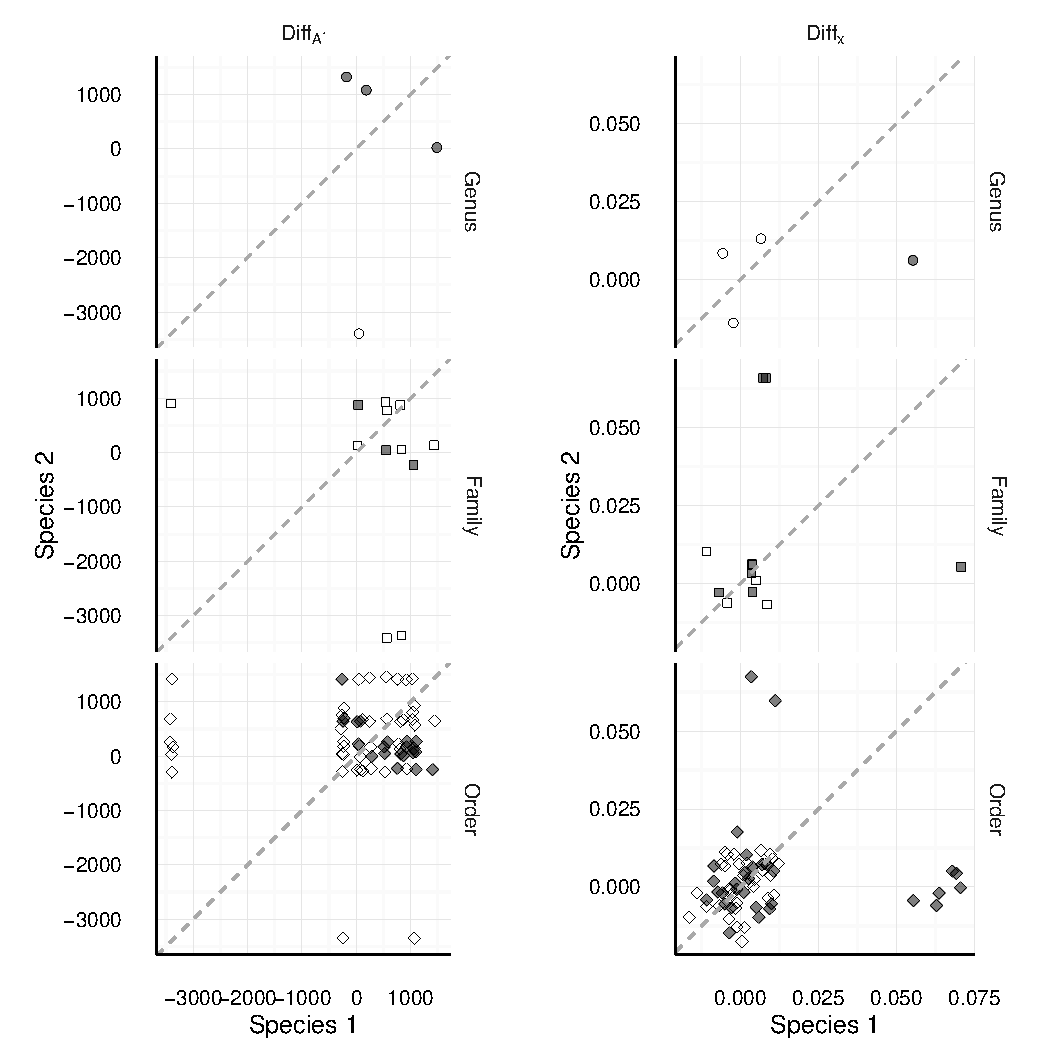
\includegraphics[width=5.5in]{figures/pairwise_astars.pdf}
\caption{Pairwise differences in two measures of size response. Each point represents a
pair of species, divided into species pairs within the same genus (top)
the same family (middle) and order (bottom). The left panel shows
differences in \(A^{*}\) values (units are ml) while the right panel
shows differences in \(x\) (slopes of logistic regression). Species
pairs which are different from a null model are shaded.}
\label{fig:pairwise}
\end{figure}

\begin{figure}[htbp]
\centering
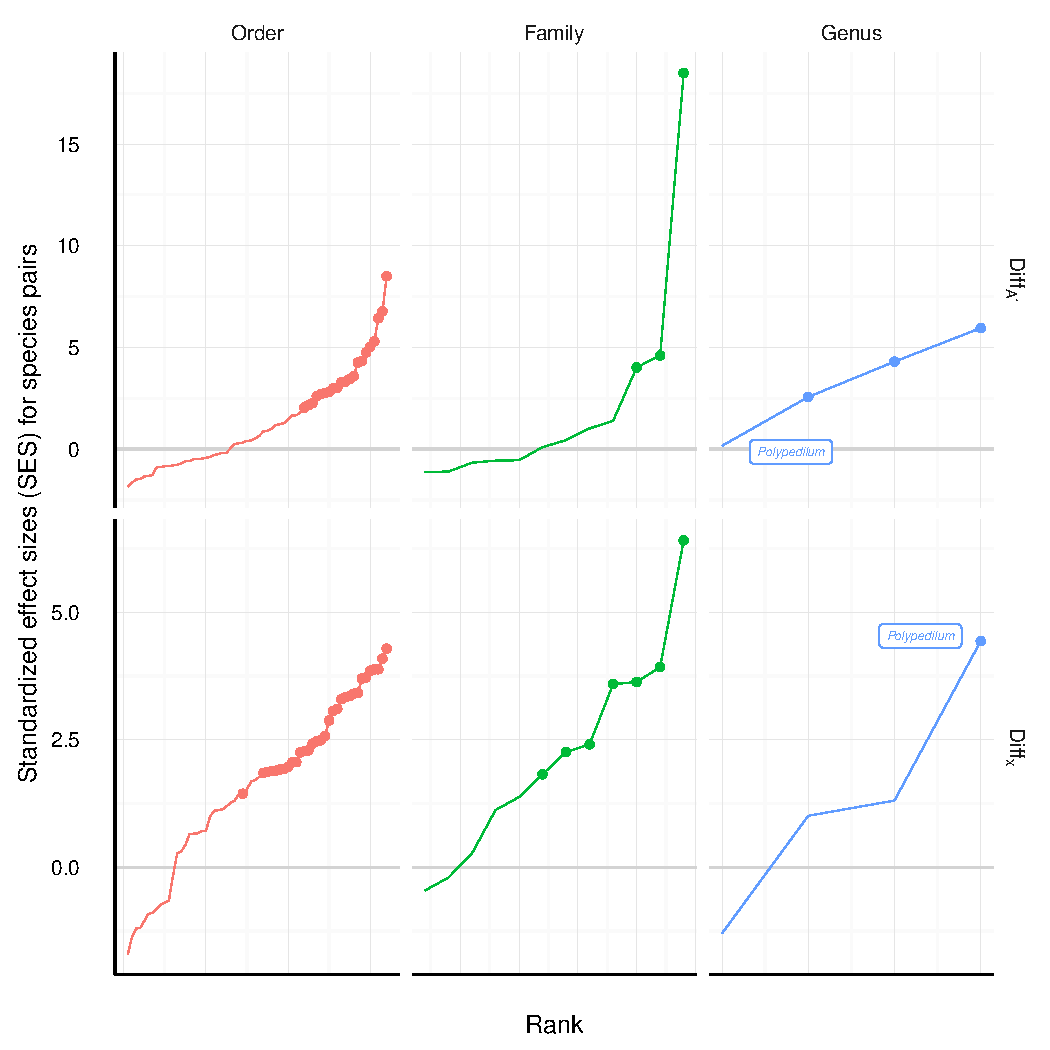
\includegraphics[width=5.5in]{figures/ses_rank.pdf}
\caption{Standardized effect sizes (SES) of pairwise differences
between species for two different measures of patch size response.
These two measures are critical patch size (\(A^{*}\)) and strength of
patch size dependency (\(x\)). Pairwise differences are shown within
each of three taxonomic levels. Significant standardized effect sizes
(randomization p-value \textless{} 0.05) are indicated with points.}
\end{figure}
